\chapter{Introduction}
The information contained in a single utterance of speech is vast. From only a few seconds of speech, we can identify a speaker's gender, age and their proximity relative to our own. The frequency and rhythms of speech can tell us about the urgency or the emotional weight of the statement. The harmonic nature, the placement of silence or noise and the prosody of the speech can then convey words and meaning. The pronunciation of these words can even tell us information about the speaker's region of birth or the circumstances of their upbringing. In only a few seconds, the human brain can receive and process this information-rich signal. 

From the 1950s onwards, researchers began working to achieve the automatic transcription of human speech. This is a task that, despite decades of research, has proven difficult to replicate. It is also the task that this thesis seeks to improve upon. The first step to understanding a speech signal is to compute the Fast Fourier Transform (FFT). The FFT enabled computers to decompose a speech signal into its frequency components efficiently. The FFTs for short overlapping windows of audio can then be computed and arranged over time. This produces a representation of the signal with frequency on the y axis, time on the x axis and frequency magnitude on the z axis. This representation is known as the spectrogram and allows us to visualise the breadth of information encoded in speech. 

In Figure~\ref{intro_fig:mel_spectrogram} we see an annotated mel-spectrogram of a short utterance of speech. A mel-spectrogram compresses frequency bands, giving greater resolution to lower frequencies where speech information is most concentrated. This utterance contains a speaker saying the words "which he understood". Below the spectrogram, we have marked some of the linguistic information contained in this speech sample. We see how words and characters can be represented in time and frequency. We further show how phonemes and their articulations, each of which produces observable patterns in the spectrum. The spectrogram demonstrates just how much information is transmitted through speech in only a few milliseconds (ms).

\begin{figure}[t]
    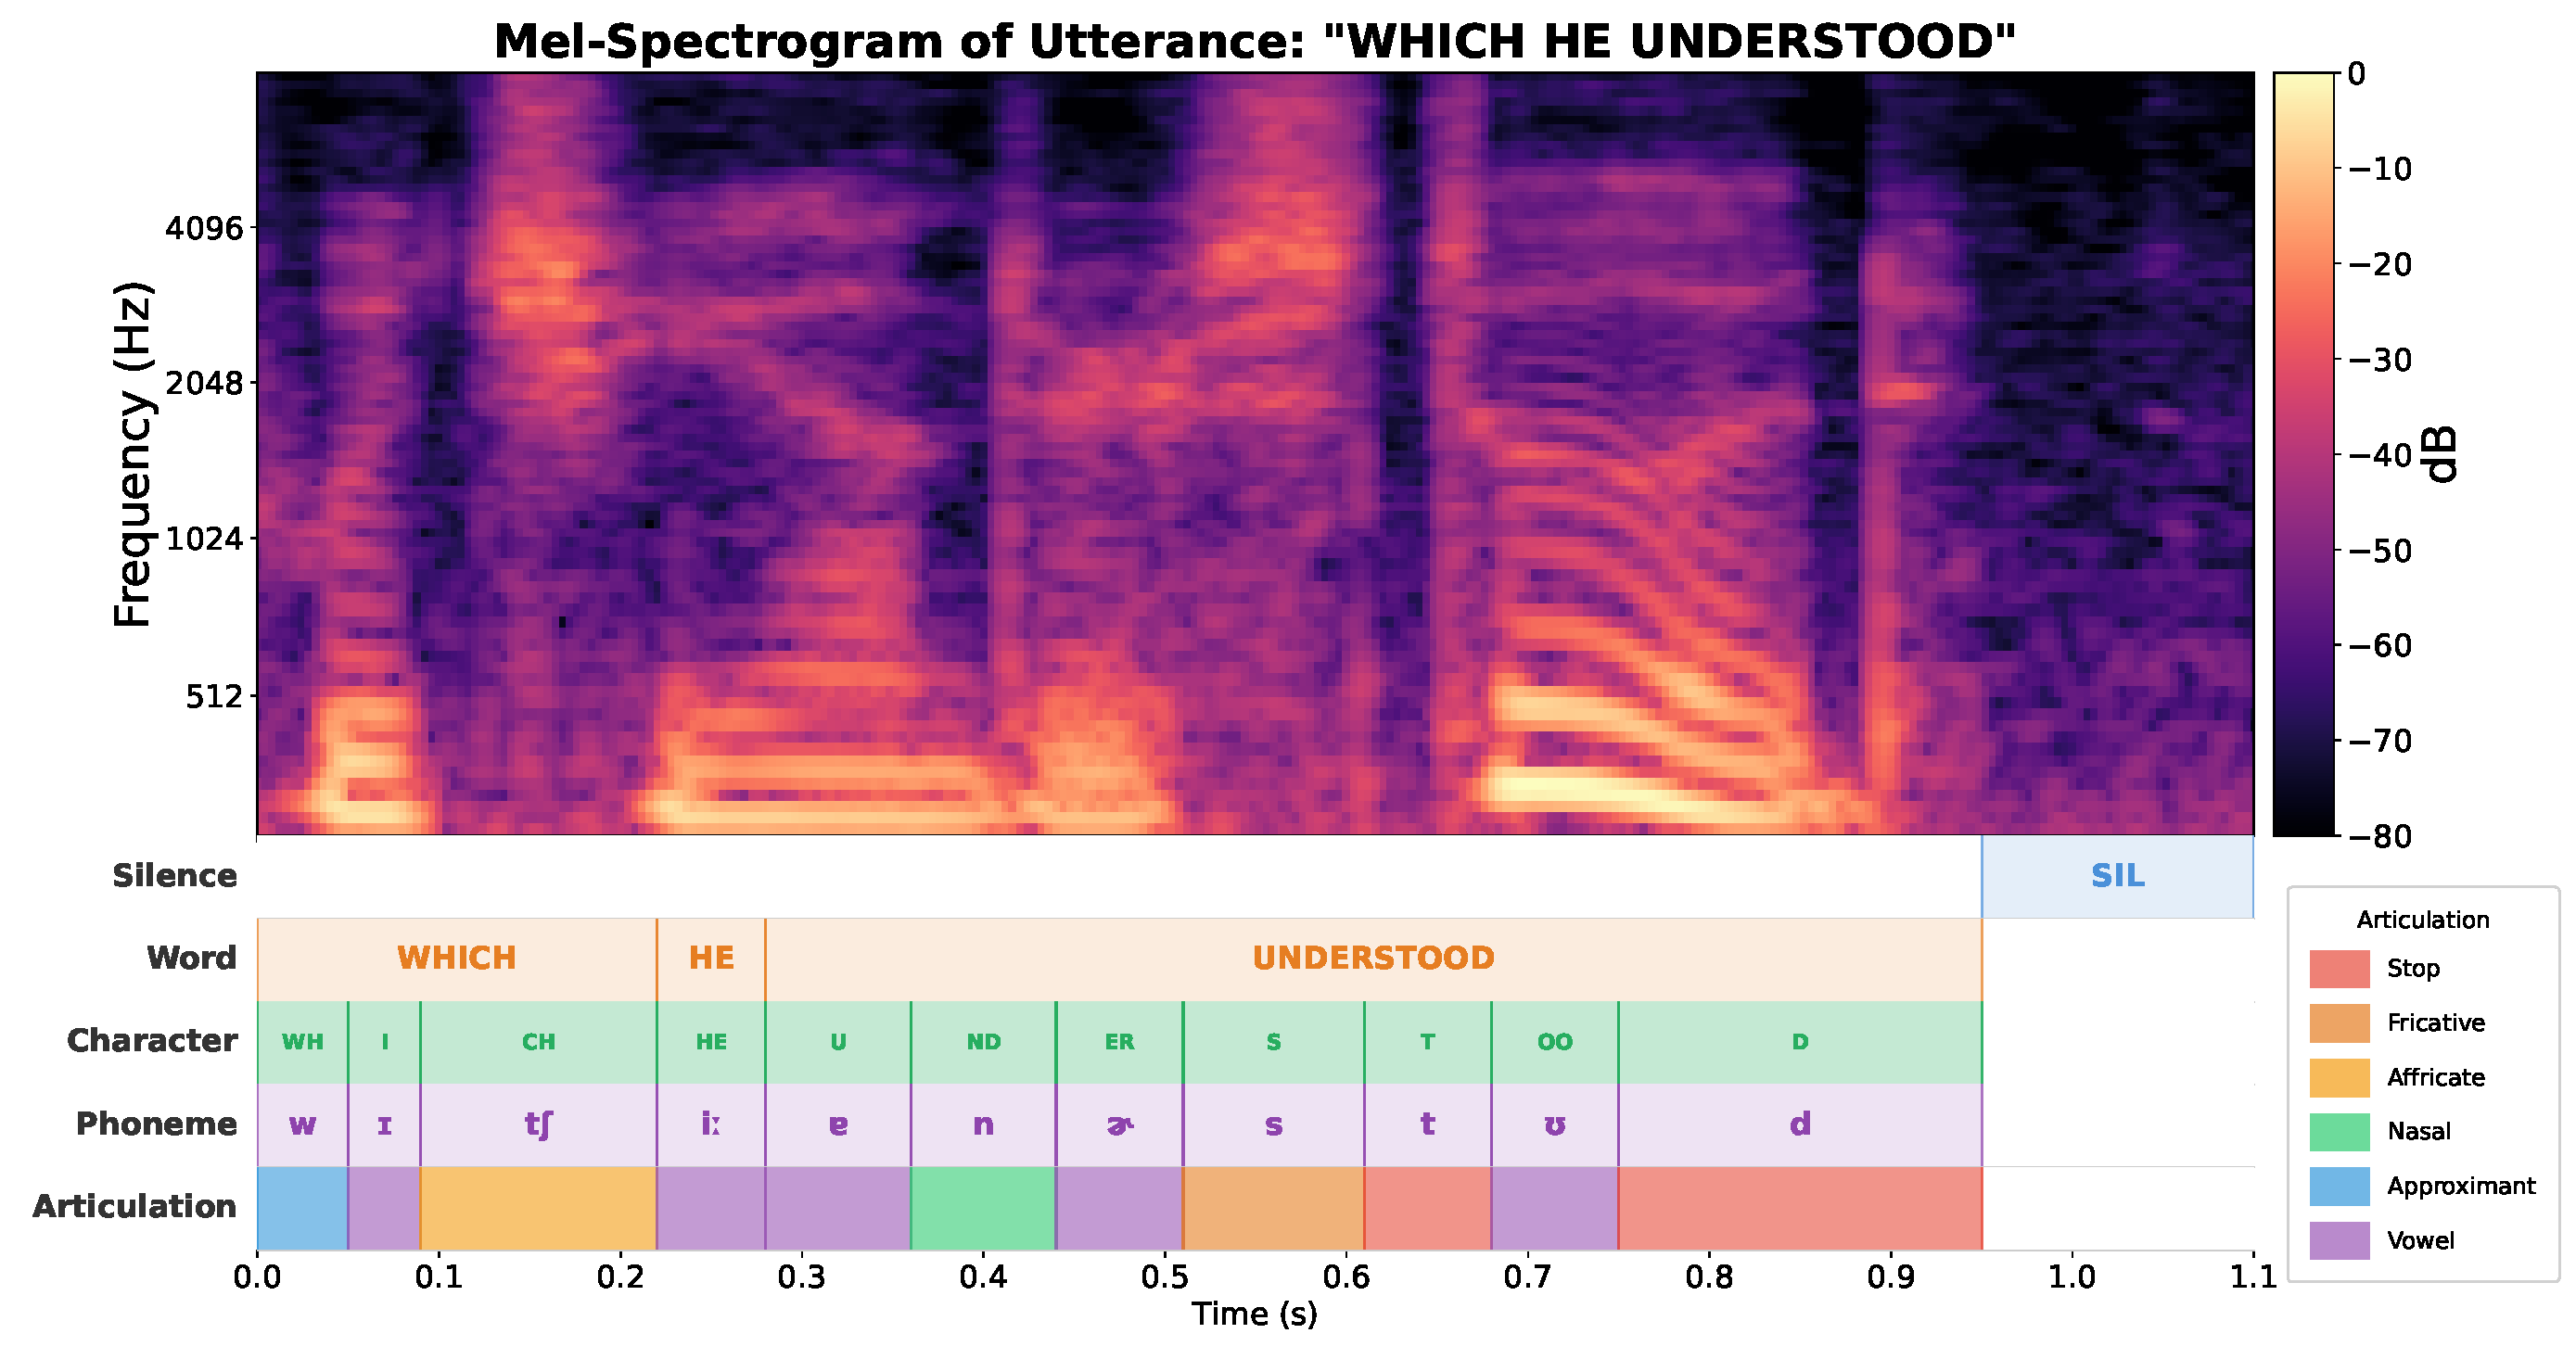
\includegraphics[width=\linewidth]{introduction/images/whichheunderstood_melspec.pdf}
    \caption{A mel-spectrogram of a section of an utterance. Here we see: word, character, phoneme and articulation level alignments. All alignments were generated with the Montreal Forced Aligner (McAuliffe et al 2017). This segment was taken from a LibriSpeech utterance (Panayotov et al. 2015).}
    \label{intro_fig:mel_spectrogram}
\end{figure}

\section{Automatic Speech Recognition}

This volume of information proved difficult for early signal processing to automatically transcribe. However, in 2014 the field of Automatic Speech Recognition (ASR) would change dramatically, with the rise of Deep Neural Networks (DNNs) \cite{hannun2014deep}. DNNs could be trained with labelled data to learn speech features. DNNs start from a random initialisation, so, are not programmed with a priori knowledge of the domain. This allows them to adapt well to the many variations of human speech such as languages, dialects and accents. DNNs were well-suited for learning ASR, wherever sufficient data was available to train them. %DNNs quickly revolutionised fields such as image processing and Natural Language Processing (NLP) \cite{citations_needed}. So when the same techniques were applied to ASR, it quickly outshone all previous approaches.

%This volume of information proved difficult for early signal processing systems to transcribe automatically. The field changed substantially with the rise of deep neural networks (DNNs), which could learn acoustic representations directly from data and reduced reliance on hand-engineered features \cite{hannun2014deep}. DNNs were well suited to automatic speech recognition, provided that sufficient training data was available.

%Early DNN architectures taught Recurrent Neural Networks (RNNs) \cite{Graves2012} to learn sequential labelled speech data using Connectionist Temporal (CTC) Loss \cite{graves2006connectionist}. 

The first DNN architectures learned speech using Connectionist Temporal Classification (CTC) Loss \cite{graves2006connectionist} and learned from thousands of hours of speech. However, CTC required human-transcribed speech data for training, but human transcription is time-consuming and expensive. So, Self-Supervised Learning (SSL) techniques were developed to learn speech without the need for expensive labelling \cite{wav2vec, hsu2021hubert}. They were combined with transformers \cite{vaswani2017attention}, which allow the parallel processing of speech frames, to achieve impressive results. This thesis explores how SSL ASR models learn and how they have been used in modern ASR.

SSL ASR models were able to vastly reduce the cost of training data by bypassing human labelling. It also expanded the number of sources from which data could be extracted. Since SSL loss functions do not have a labelled objective, training must be split into 2 stages: pretraining and fine-tuning. The pretraining stage is done with SSL and then the model is fine-tuned to a labelled objective, such as speech transcriptions, with CTC. To maximise the benefits of SSL, training on large datasets for long periods is done during pretraining. Unlabelled data cannot be utilised in fine-tuning. There are many resources for unlabeled or semi-labelled data, so including them can greatly expand the size of the data pool. The fine-tuning dataset can then be much smaller than the pretraining dataset, since the bulk of learning has already been done.

By making pretrained SSL models open-source\footnote{\hyperlink{https://huggingface.co/facebook/wav2vec2-base}{huggingface.co/facebook/wav2vec2-base}}, they could be fine-tuned to a variety of different datasets. With pretraining, a small amount of fine-tuning data could produce accurate results in multiple speech domains. Some domains, such as small languages or dialects, did not have the large datasets required to train an ASR model from scratch. We refer to these domains as being low-resource. For low-resource domains, SSL pretraining provided an adaptable baseline model that could be fine-tuned to achieve impressive results.

However, it was quickly found that the data used in pretraining has an impact on downstream performance. Most SSL models were pretrained on data from a single language, monolingual pretraining. If the model was fine-tuned to the same language or a related language as the pretraining data, the results could be exceptional. We call this matched-language or related-language fine-tuning. However, if the fine-tuning language was not the same as the pretraining language, it would negatively impact performance. We refer to this as mismatched-language fine-tuning.

The solution, therefore, was to make SSL ASR models multilingual \cite{XLSR-53, whisper}. By pretraining on many different languages, these models were able to substantially improve fine-tuning accuracy for low-resource languages. However, the more languages that were added to pretraining, the worse the performance could be for individual languages. When the size of each model is increased, this trade-off can be offset \cite{babu2021xlsr}. However, as the model size increases the compute power required for both the pretraining and fine-tuning stages also increases. This reduces the benefits of pretraining for low-resource languages. 

This is the point in ASR research that we find ourselves as of the writing of this thesis. The contributions to knowledge in this thesis, therefore, aim to expand our understanding of multilingual SSL ASR. We hope that by contributing, we can help to improve ASR for low-resource languages. These contributions are outlined throughout the rest of this chapter.

%In order to contribute knowledge to the field of ASR, we first explore how SSL ASR models learn speech. We first outline everything currently known about SSL ASR learning. Then we perform experiments to further our knowledge and improve the current performance of multilingual SSL ASR models. We finally suggest how these findings can be used going forward. With these aims in mind, we hope that accurate and efficient ASR can be made available to many more languages and many more people in the future.  


%\section{Thesis Statement}

\section{Research Questions}\label{intro_sec:research_questions}
\iffalse
\begin{itemize}
    \item What do SSL models learn from multilingual data?
    \item We know that SSL models learn aspects of each language but do they learn them equally?
    \item How does the balance of languages in pretraining affect language learning?
    \item Do SSL models learn languages independently?
    \item We know that the XLSR-53 quantizer groups features, so some features at least appear to be language-dependent, but are all of them? 
    \item How does SSL learn imbalanced languages? 
    \item Does SSL rely more on high-resource languages and share more features when learning low-resource languages or do low-resource languages simply suffer?
    \item 
    
\end{itemize}
\fi

This thesis seeks to understand how SSL ASR learn the features of multilingual data. This understanding can then be used to improve ASR for languages across the world. To achieve this, we seek to answer the following research questions:%\newline

%\hl{Do I want to change this to be more like Sam's?}

\begin{enumerate}[start=1,label={\bfseries RQ\arabic*:}]%[RQ*]%[start=0,label={\textbf{RQ}*:}]
    \item How does the balance in hours between different languages included in multilingual SSL pretraining data affect language learning?
    %\begin{enumerate}[start=1,label={\bfseries RQ1.\arabic*:}]
        %\item What does an SSL model learn when a language is low-resource in pretraining?
        %\item Does an imbalance between the language have a negative affect on multilingual learning?
        %\item Does the proportion of data for a language in pretraining affect how well that is learned during pretraining?
        %\item When the languages in the pretraining data are not balanced equally, how much does the model learn about each one?
        \item Do multilingual ASR models use information from related languages learned in pretraining, when performing monolingual fine-tuning?
        %\item How do high-resource pretraining languages interact with the learning of low-resource languages during pretraining?
        %\item Are all languages learned equally in multilingual pretraining, and if not 
    %\end{enumerate}
    \item How do multilingual models learn multilingual phonetic features?
    %\begin{enumerate}[start=1,label={\bfseries RQ2.\arabic*:}]
        \item Do multilingual SSL models learn shared phoneme representations, or do they learn language-specific phoneme realisations separately?
        %\item Articulations are learned to different degrees in English pretraining, is this consistent in multilingual pretraining? \hl{I have removed this from the conclusion for the momemnt. I could change this refernce unseen languges instead...}
        \item How do the languages in pretraining relate to the downstream accuracy of unseen languages?
        \item How does the balance of languages in pretraining affect how each articulation class is learned across languages?%\newline
        %\item Each articulation is learned to a different degree of accuracy in English monolingual pretraining but does this apply in multilingual pretraining?\newline
        %\item Are there any phonetic features that are better shared across languages than others?
        %\item Are all phonetic features language-specific or does the model share any latent space?
    %\end{enumerate}
\end{enumerate}
%\textbf{RQ1} How does the balance in hours of between languages in SSL pretraining affect language learning?


Chapter~\ref{chapter4} primarily addresses \textbf{RQ1} and \textbf{RQ2}. In this chapter, we explore the language-specific subnetworks in the multilingual SSL ASR model XLS-R. We look at which of these language-specific subnetworks are used when fine-tuning. We identify which subnetworks have the lowest Character Error Rates (CERs) across languages. We also isolate languages that are low-resource in pretraining or absent altogether. We then test which language-specific subnetwork produces the lowest CER for these languages. By identifying how subnetworks interact with different languages, we address these research questions. 

Chapter~\ref{chapter5} continues the investigation of language balance in multilingual pretraining, further exploring \textbf{RQ2}. In this chapter, we pretrain 7 multilingual SSL ASR models with different ratios of English and Spanish data. We explore how the ratio between pretraining languages affects fine-tuned error rates. We then probe the models and measure phoneme accuracy and address \textbf{RQ4}. We examine how language-specific realisations of the same phonemes are recognised in each model, answering \textbf{RQ4}. We extend this analysis to measuring the accuracy of phonemes realised in languages unseen in pretraining, which addresses \textbf{RQ5}. We then group phonemes by their Manner of Articulation (MoA) classes and explore how articulations are learned during multilingual pretraining. These findings allow us to answer \textbf{RQ6}.

\newpage
\section{Thesis Outline}
This section gives a high-level outline for each chapter included in this thesis. 

\subsubsection{Chapter~\ref{Chapter2_LR}: Literature Review}
Chapter~\ref{Chapter2_LR} gives a detailed description of the literature that underpins the research throughout this thesis. Section~\ref{lr_sec:asr_early_dnns} covers early uses of DNNs on ASR. We explain the transformer architecture and how processing sequences in parallel changed ASR. Section~\ref{lr_sec:wav2vec2} explains the wav2vec 2.0 SSL ASR model \cite{wav2vec}. We describe the contrastive loss function, the quantizer and how wav2vec 2.0 learns. Section~\ref{lr_sec:multilingual_ssl} details multilingual SSL ASR. We examine the relationship between ASR performance and model size when pretraining on multilingual and monolingual datasets. In Section~\ref{lr_sec:model_compression}, we describe common model compression techniques and go into depth on weight pruning. We explore how language-specific subnetworks can be found within large multilingual ASR models. Section~\ref{lr_sec:model_analysis} details the approaches researchers have taken to analysing SSL ASR models. We cover statistical layer analysis as well as layer analysis through probing. We then review all studies on phoneme and articulation information learned by SSL ASR models. Finally, Section~\ref{lr_sec:datasets_models} presents the models, datasets and training regimes used in the experiments throughout this thesis.

\subsubsection{Chapter~\ref{chapter4}: Language Bias in Self-Supervised Learning for Automatic Speech Recognition}
Chapter~\ref{chapter4} analyses the weight distribution of the multilingual SSL ASR model XLS-R \cite{babu2021xlsr}. Section~\ref{pru_sec:introduction} and section~\ref{pru_sec:background} outline recent advances in multilingual SSL ASR. They cover the size of XLS-R and how model compression techniques aim to reduce the size. They cover how weight pruning can uncover language-specific subnetworks. Section~\ref{pru_sec:experimental_design} outlines our experimental procedure. We describe the architecture of XLS-R and the data it was pretrained on. We detail our pruning strategy and our method for identifying language-specific subnetworks. In Section~\ref{pru_sec:experimental_results}, we identify multiple language-specific subnetworks within XLS-R. We then test the fine-tuned CER on matched-languages and mismatched-languages. We analyse their weight distributions and where language-specific subnetworks overlap. Then, in section~\ref{pru_sec:discussion} and Section~\ref{pru_sec:conclusion} we discuss our findings. 

\newpage
\subsubsection{Chapter~\ref{chapter5}: Data Balance and Learning in Multilingual SSL}
In Chapter~\ref{chapter5}, we measure how the ratio between the number of hours in each pretraining language relates to the downstream performance of multilingual SSL ASR models. Section~\ref{ed_sec:introduction} and section~\ref{ed_sec:background} outline the trade-off between multilingual and monolingual SSL pretraining. This section also covers methods used to analyse how SSL ASR models learn speech, including statistical layer analysis and layer probing. In section~\ref{ed_sec:experimental_design}, we outline our experimental methodology. We describe each of our pretraining, fine-tuning and layer probing strategies. We then outline how we will use these strategies to understand how SSL learns multilingual phonetic features. In section~\ref{ed_sec:experimental_results}, we present our results. We show how the ratio between pretraining languages relates directly to fine-tuned error rates. We then prove that individual phonemes are learned as language-specific realisations. We finally present phoneme accuracy at an articulation level. WWe find that MoA classes are not learned equally across languages and several factors can contribute to high MoA class accuracy. Finally, in section~\ref{ed_sec:discussion} and section~\ref{ed_sec:conclusion} we discuss our findings. 


\subsubsection{Chapter \ref{Chapter6}: Conclusion}
In Chapter~\ref{Chapter6} we outline the findings and contributions raised in this thesis. In section~\ref{conc_sec:summary} we summarise Chapter~\ref{chapter4} and Chapter~\ref{chapter5} and whether this thesis answers the research questions. In section~\ref{conc_sec:limitations} we outline some limitations to the experiments in this thesis. We reflect on how those limitations affect our interpretation of the findings in this thesis. In section~\ref{conc_sec:future_work}, we outline the future work that could be done based on the contributions of this thesis. Finally, in section~\ref{conc_sec:final_remark} we outline the final remarks on this thesis.

%\section{Contributions}
\section{Research Contributions}
\iffalse
\begin{itemize}
    \item Chapter 4
    \item Contributions to Language-specific subnetworks
    \item identifying that 80\% of the subnetworks overlap
    \item Identifying that new languages learn from English weights
    \item Identifying that XLS-R can be reduced in size by up to 60\% with no impact on WER and 70\% with little impact
\end{itemize}

\begin{itemize}    
    \item Chapter 5
    \item Identifying exactly how much multilingual data affects finetuned WER
    \item How well phonemes that exist in pretraining are recognised by the model
    \item How well phonemes that don't exist in pretraining are recognised
    \item How language affects phonemes, does a phoneme that exists in both languages get high accuracy or has the model learned realisations separately?
    \item How different MoA are understood by multilingual SSL models
    \item How the number of interval counts in pretraining relates to MoA class accuracy
    \item How phoneme interval counts in pretraining and probe training relate to accuracy
    \item How interval counts in a class relate to unseen phoneme accuracy.
\end{itemize}
\fi

%Here we summarise the contributions to knowledge as follows:

\subsubsection{Contributions relating to Chapter~\ref{chapter4}.}\label{intro_subsec:contributions}

The contributions outlined in this chapter were presented at the IEEE, Spoken Language Technology (SLT) conference, in Macau in 2024. 

\begin{enumerate}
    \item \textbf{Sparsity in Multilingual XLS-R}

    We compare the sparsity that different language-specific subnetworks can be pruned to without increasing the error. We show in Chapter~\ref{chapter4} that, for all languages, XLS-R can be pruned to 50\% sparsity without any increase in the error rate. We further show that, for all languages, XLS-R can be pruned to 70\% without a significant increase in error.

    \item \textbf{Subnetwork Performance}
    
    Previous studies had shown that fine-tuning to matched-language subnetworks produced the lowest CER. However, for XLS-R, this is not true. The best performing subnetwork comes from English. English is the language that contributes the most hours to the pretraining data. We compare the CER produced by each language-specific subnetwork, at >=70\% sparsity, when fine-tuned to multiple languages. We find that the English language-specific subnetwork produces the lowest CER for all languages. This is true even when compared to matched-language fine-tuning for other languages. 

    %\item \textbf{Subnetwork Adaptability}

    %We show that pruning with the English language-specific subnetwork can lower CER even after fine-tuning XLS-R to a language other than English. We fine-tune XLS-R to Spanish and prune with the English subnetwork. We show that this pruned model produces lower CER for English, Asturian and Xhosa, when compared to pruning the same model to the Spanish subnetwork. The matched-language, Spanish, is the only language that increases in CER.


    %With this finding we test the performance of fine-tuned subnetworks on related and unrelated languages. We fine-tune Spanish and English subnetworks on 4 languages: English, Spanish, Asturian and Xhosa.  Spanish, Catalan and Asturian are all closely related Romance languages originating in Spain. and the CER\thoughts{Need to define CER/WER earlier} 

    \item \textbf{The Overlap Between language-specific subnetworks}

    We test the Intersection Over Union (IOU) between language-specific subnetworks. The IOU measures how many weights each subnetworks share. Previous studies showed language-specific subnetworks to have a >90\% IOU for models trained from scratch. For XLS-R, we show the IOU is always between 80\% and 90\%. We further show that the English subnetwork had the highest IOU with the pretrained model, before fine-tuning. Previous studies had not measured how language-specific subnetworks generated from related languages interact. So, finally, we show that Asturian and Catalan subnetworks have a higher IOU with the English subnetwork than the Spanish subnetwork.
    
\end{enumerate}

\subsubsection{Contributions relating to Chapter~\ref{chapter5}.} 

Prior studies have shown that wav2vec 2.0 learns phonemes and manner of articulation during pretraining. The contributions in this chapter explore how multilingual pretraining affects phonetic feature learning. The contributions in this chapter have yet to be published.

\begin{enumerate}
    \item \textbf{How language balance in pretraining reflects Error Rate}

    Previous studies show that monolignual matched-language pretraining and multilingual related language pretraining can decrease fine-tuned CER. Multilingual mismatched pretraining can increase CER when compared. We prove that the ratio of matched to mismatched languages also relates directly to fine-tuned CER. As matched-language data is increased in pretraining, fine-tuned error reduces proportionally. Inversely, as the amount of mismatched data is increased, the CER increases proportionally. We further prove that this relationship is also true for related languages. As related language data in pretraining increases, fine-tuned CER reduces proportionally.

    \newpage
    \item \textbf{Phonemes are learned as language-specific realisations}

    We find that language-specific phoneme realisations are learned separately in pretraining. As matched-language data is increased in pretraining, matched-language phoneme accuracy increases proportionally. As the mismatched-language increases, mismatched-language phoneme accuracy decreases proportionally. We also test unseen languages, those that are not included in pretraining. Unseen related language phonemes that exist in pretraining have a higher average accuracy than phonemes that do not exist in pretraining. This is true for unseen mismatched language phonemes as well.

    %\item \textbf{How language balance in pretraining reflects Phoneme Accuracy}

    \item \textbf{How multilingual pretraining learns articulation}

    previous studies have shown that SSL ASR learn articulations, however multilingual articulations have not been explored. We find that multilingual SSL ASR does not learn MoA classes equally. Multiple factors can contribute to how well multilingual SSL has learned an articulation class. For each class the dominant factor can be different. These factors include: pretraining class exposure, the ratio between pretraining languages and the language a phoneme is spoken in. 
    
    %In some cases a MoA class with high exposure in pretraining can have high average accuracy. In other cases one of the pretraining languages can produce higher accuracy for a class than the other. This can be true even for phonemes spoken in unseen languages. The ratio between the pretraining language hours can then further impact this class accuracy. We present these and other findings on multilingual MoA accuracy.
    
    %For example, vowels are high-resource across all language ratios in pretraining. Vowels also have a high average accuracy across all languages. Fricatives that do not appear in either pretraining language have higher accuracy when compared to other MoA classes. Spanish trills in pretraining do not increase Polish trill accuracy. We present these and other findings on multilingual MoA accuracy.

\end{enumerate}

\section{Publications}

%\textbf{Storey, E.}, Harte, N., Bell, P. (2024).

\begin{enumerate}
    \item \textbf{Storey, E.}, Harte, N., and Bell, P. (2024) "Language Bias in Self-Supervised Learning For Automatic Speech Recognition," \textit{IEEE Spoken Language Technology Workshop (SLT)}, Macao, 2024, pp. 37-42, doi:10.1109/SLT61566.2024.10832268.
\end{enumerate}

\nomenclature[A]{CTC}{Connectionist Temporal Classification}
\nomenclature[A]{ASR}{Automatic Speech Recognition}
\nomenclature[A]{DNN}{Deep Neural Network}
\nomenclature[A]{SSL}{Self-Supervised Learning}
